\documentclass[11pt]{article}
\usepackage{amsmath}
\usepackage{fancyhdr}
\usepackage{hyperref}
\usepackage{graphicx}
\newcommand{\compactlist}{\setlength{\itemsep}{0pt} \setlength{\parskip}{0pt} \setlength{\leftskip}{-1em}}
\usepackage[top=0.9in, bottom=0.8in, left=0.9in, right=0.9in]{geometry}

\lhead{MATH 4263/5373}
\rhead{Sep. 10, 2019}
\chead[RE]{Fixed-point iterations: II}
\cfoot{}
\rfoot{}%Code for figure and report is (not yet) available in the class folder.}
\pagestyle{fancy}

\begin{document}

Consider the root-finding problem \(3x^2-e^x = 0\). It has a few different, but equivalent, fixed-point problems.
\begin{align}
g_1(x) & = \pm\sqrt{\dfrac{e^x}{3}} = x\\
g_2(x) & = \ln(3x^2) = x\\
g_3(x) & = 3x^2 - e^x + x = x
\end{align}
Unfortunately these differ with regard to theory of fixed-point iterations. In particular, keep in mind
\begin{description}
\item[for existence:] the trapping region \(g\in[a,b]\) for \(x\in[a,b]\)
\item[for uniqueness:] the slope criterion \(0<|g'(x)|<1\)
\end{description}

The first function, \(g_1(x)\) is able to capture two of the three points of interest, with nicely trapped solutions and small derivatives on those intervals. It does fail to capture the third (rightmost) root, where the slope exceeds one (see Fig.~\ref{fig::g1}). Though our intervals cannot include \(x=0\), \(g_2(x)\) works well for the largest root, where the derivative is small and the appropriate trapping region can be constructed (see Fig.~\ref{fig::g2}). The simplest formulation algebraically is \(g_3(x)\), yet this has by far the worst characteristics with respect to the fixed-point theory for existence and uniqueness (see Fig.~\ref{fig::g3}). It is difficult to constrict suitable trapping regions and there are only narrow ranges for which the derivative is appropriately bounded in magnitude. 

\begin{figure}[h!]
\begin{minipage}{0.48\textwidth}
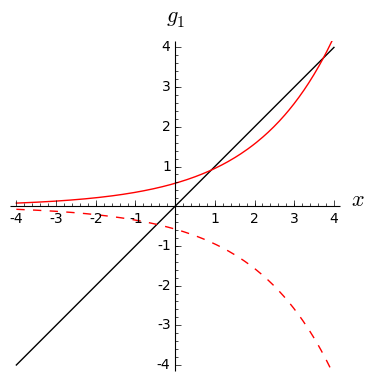
\includegraphics[width=\textwidth]{g1.png}
\end{minipage}
\begin{minipage}{0.48\textwidth}
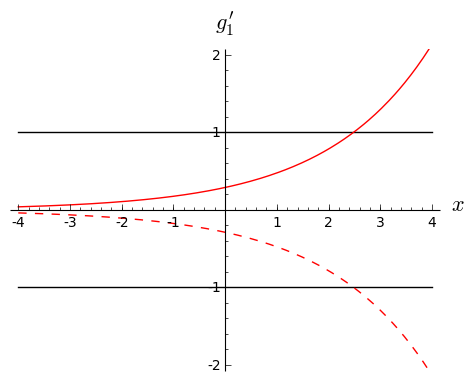
\includegraphics[width=\textwidth]{g1p.png}
\end{minipage}
\caption{Two functions that give rise to fixed-point problems. Dotted corresponds to the negative value of the square root and the solid line corresponds to the positive value. Left: intersections of each with the black \(1:1\) line indicate fixed points. Right: values between \(-1\) and \(1\) indicate that a fixed point, if it exists, is unique.}\label{fig::g1}
\end{figure}

\begin{figure}[h!]
\begin{minipage}{0.48\textwidth}
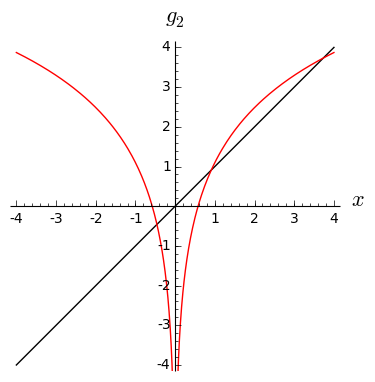
\includegraphics[width=\textwidth]{g2.png}
\end{minipage}
\begin{minipage}{0.48\textwidth}
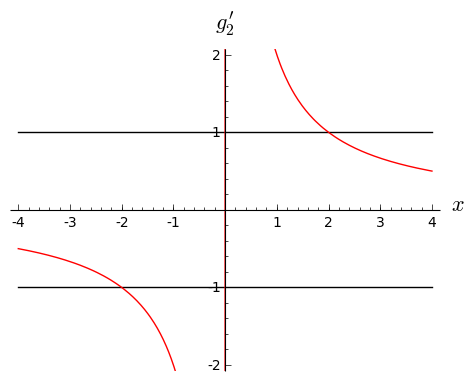
\includegraphics[width=\textwidth]{g2p.png}
\end{minipage}
\caption{Left: intersections with the black \(1:1\) line indicate fixed points. Right: values between \(-1\) and \(1\) indicate that a fixed point, if it exists, is unique. Notice that the smaller the value of the fixed point, the steeper the function \(g_2(x)\).}\label{fig::g2}
\end{figure}

\begin{figure}[b!]
\begin{minipage}{0.48\textwidth}
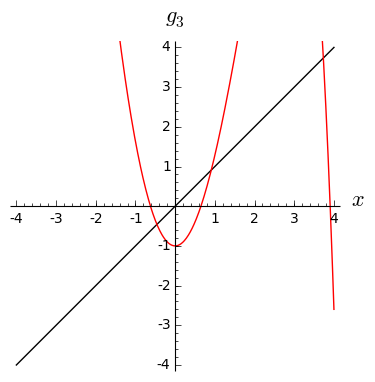
\includegraphics[width=\textwidth]{g3.png}
\end{minipage}
\begin{minipage}{0.48\textwidth}
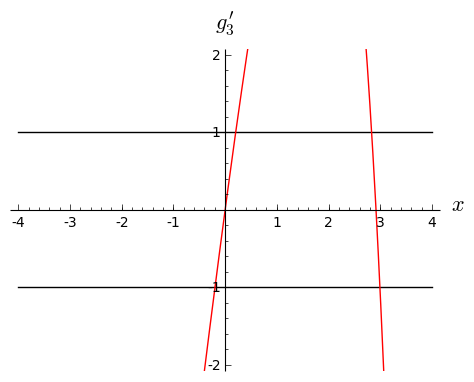
\includegraphics[width=\textwidth]{g3p.png}
\end{minipage}
\caption{Left: intersections with the black \(1:1\) line indicate fixed points. Right: values between \(-1\) and \(1\) indicate that a fixed point, if it exists, is unique.}\label{fig::g3}
\end{figure}

\end{document}














